
%% bare_conf.tex
%% V1.3
%% 2007/01/11
%% by Michael Shell
%% See:
%% http://www.michaelshell.org/
%% for current contact information.
%%
%% This is a skeleton file demonstrating the use of IEEEtran.cls
%% (requires IEEEtran.cls version 1.7 or later) with an IEEE conference paper.
%%
%% Support sites:
%% http://www.michaelshell.org/tex/ieeetran/
%% http://www.ctan.org/tex-archive/macros/latex/contrib/IEEEtran/
%% and
%% http://www.ieee.org/

%%*************************************************************************
%% Legal Notice:
%% This code is offered as-is without any warranty either expressed or
%% implied; without even the implied warranty of MERCHANTABILITY or
%% FITNESS FOR A PARTICULAR PURPOSE! 
%% User assumes all risk.
%% In no event shall IEEE or any contributor to this code be liable for
%% any damages or losses, including, but not limited to, incidental,
%% consequential, or any other damages, resulting from the use or misuse
%% of any information contained here.
%%
%% All comments are the opinions of their respective authors and are not
%% necessarily endorsed by the IEEE.
%%
%% This work is distributed under the LaTeX Project Public License (LPPL)
%% ( http://www.latex-project.org/ ) version 1.3, and may be freely used,
%% distributed and modified. A copy of the LPPL, version 1.3, is included
%% in the base LaTeX documentation of all distributions of LaTeX released
%% 2003/12/01 or later.
%% Retain all contribution notices and credits.
%% ** Modified files should be clearly indicated as such, including  **
%% ** renaming them and changing author support contact information. **
%%
%% File list of work: IEEEtran.cls, IEEEtran_HOWTO.pdf, bare_adv.tex,
%%                    bare_conf.tex, bare_jrnl.tex, bare_jrnl_compsoc.tex
%%*************************************************************************

% *** Authors should verify (and, if needed, correct) their LaTeX system  ***
% *** with the testflow diagnostic prior to trusting their LaTeX platform ***
% *** with production work. IEEE's font choices can trigger bugs that do  ***
% *** not appear when using other class files.                            ***
% The testflow support page is at:
% http://www.michaelshell.org/tex/testflow/



% Note that the a4paper option is mainly intended so that authors in
% countries using A4 can easily print to A4 and see how their papers will
% look in print - the typesetting of the document will not typically be
% affected with changes in paper size (but the bottom and side margins will).
% Use the testflow package mentioned above to verify correct handling of
% both paper sizes by the user's LaTeX system.
%
% Also note that the "draftcls" or "draftclsnofoot", not "draft", option
% should be used if it is desired that the figures are to be displayed in
% draft mode.
%
\documentclass[conference]{IEEEtran}
% Add the compsoc option for Computer Society conferences.
%
% If IEEEtran.cls has not been installed into the LaTeX system files,
% manually specify the path to it like:
% \documentclass[conference]{../sty/IEEEtran}





% Some very useful LaTeX packages include:
% (uncomment the ones you want to load)


% *** MISC UTILITY PACKAGES ***
%
%\usepackage{ifpdf}
% Heiko Oberdiek's ifpdf.sty is very useful if you need conditional
% compilation based on whether the output is pdf or dvi.
% usage:
% \ifpdf
%   % pdf code
% \else
%   % dvi code
% \fi
% The latest version of ifpdf.sty can be obtained from:
% http://www.ctan.org/tex-archive/macros/latex/contrib/oberdiek/
% Also, note that IEEEtran.cls V1.7 and later provides a builtin
% \ifCLASSINFOpdf conditional that works the same way.
% When switching from latex to pdflatex and vice-versa, the compiler may
% have to be run twice to clear warning/error messages.






% *** CITATION PACKAGES ***
%
%\usepackage{cite}
% cite.sty was written by Donald Arseneau
% V1.6 and later of IEEEtran pre-defines the format of the cite.sty package
% \cite{} output to follow that of IEEE. Loading the cite package will
% result in citation numbers being automatically sorted and properly
% "compressed/ranged". e.g., [1], [9], [2], [7], [5], [6] without using
% cite.sty will become [1], [2], [5]--[7], [9] using cite.sty. cite.sty's
% \cite will automatically add leading space, if needed. Use cite.sty's
% noadjust option (cite.sty V3.8 and later) if you want to turn this off.
% cite.sty is already installed on most LaTeX systems. Be sure and use
% version 4.0 (2003-05-27) and later if using hyperref.sty. cite.sty does
% not currently provide for hyperlinked citations.
% The latest version can be obtained at:
% http://www.ctan.org/tex-archive/macros/latex/contrib/cite/
% The documentation is contained in the cite.sty file itself.






% *** GRAPHICS RELATED PACKAGES ***
%
\ifCLASSINFOpdf
  \usepackage[pdftex]{graphicx}
  % declare the path(s) where your graphic files are
  % \graphicspath{{../pdf/}{../jpeg/}}
  % and their extensions so you won't have to specify these with
  % every instance of \includegraphics
  % \DeclareGraphicsExtensions{.pdf,.jpeg,.png}
\else
  % or other class option (dvipsone, dvipdf, if not using dvips). graphicx
  % will default to the driver specified in the system graphics.cfg if no
  % driver is specified.
  \usepackage[dvips]{graphicx}
  % declare the path(s) where your graphic files are
  \graphicspath{{../eps/}}
  % and their extensions so you won't have to specify these with
  % every instance of \includegraphics
  \DeclareGraphicsExtensions{.eps}
\fi
% graphicx was written by David Carlisle and Sebastian Rahtz. It is
% required if you want graphics, photos, etc. graphicx.sty is already
% installed on most LaTeX systems. The latest version and documentation can
% be obtained at: 
% http://www.ctan.org/tex-archive/macros/latex/required/graphics/
% Another good source of documentation is "Using Imported Graphics in
% LaTeX2e" by Keith Reckdahl which can be found as epslatex.ps or
% epslatex.pdf at: http://www.ctan.org/tex-archive/info/
%
% latex, and pdflatex in dvi mode, support graphics in encapsulated
% postscript (.eps) format. pdflatex in pdf mode supports graphics
% in .pdf, .jpeg, .png and .mps (metapost) formats. Users should ensure
% that all non-photo figures use a vector format (.eps, .pdf, .mps) and
% not a bitmapped formats (.jpeg, .png). IEEE frowns on bitmapped formats
% which can result in "jaggedy"/blurry rendering of lines and letters as
% well as large increases in file sizes.
%
% You can find documentation about the pdfTeX application at:
% http://www.tug.org/applications/pdftex





% *** MATH PACKAGES ***
%
%\usepackage[cmex10]{amsmath}
% A popular package from the American Mathematical Society that provides
% many useful and powerful commands for dealing with mathematics. If using
% it, be sure to load this package with the cmex10 option to ensure that
% only type 1 fonts will utilized at all point sizes. Without this option,
% it is possible that some math symbols, particularly those within
% footnotes, will be rendered in bitmap form which will result in a
% document that can not be IEEE Xplore compliant!
%
% Also, note that the amsmath package sets \interdisplaylinepenalty to 10000
% thus preventing page breaks from occurring within multiline equations. Use:
%\interdisplaylinepenalty=2500
% after loading amsmath to restore such page breaks as IEEEtran.cls normally
% does. amsmath.sty is already installed on most LaTeX systems. The latest
% version and documentation can be obtained at:
% http://www.ctan.org/tex-archive/macros/latex/required/amslatex/math/





% *** SPECIALIZED LIST PACKAGES ***
%
%\usepackage{algorithmic}
% algorithmic.sty was written by Peter Williams and Rogerio Brito.
% This package provides an algorithmic environment fo describing algorithms.
% You can use the algorithmic environment in-text or within a figure
% environment to provide for a floating algorithm. Do NOT use the algorithm
% floating environment provided by algorithm.sty (by the same authors) or
% algorithm2e.sty (by Christophe Fiorio) as IEEE does not use dedicated
% algorithm float types and packages that provide these will not provide
% correct IEEE style captions. The latest version and documentation of
% algorithmic.sty can be obtained at:
% http://www.ctan.org/tex-archive/macros/latex/contrib/algorithms/
% There is also a support site at:
% http://algorithms.berlios.de/index.html
% Also of interest may be the (relatively newer and more customizable)
% algorithmicx.sty package by Szasz Janos:
% http://www.ctan.org/tex-archive/macros/latex/contrib/algorithmicx/




% *** ALIGNMENT PACKAGES ***
%
%\usepackage{array}
% Frank Mittelbach's and David Carlisle's array.sty patches and improves
% the standard LaTeX2e array and tabular environments to provide better
% appearance and additional user controls. As the default LaTeX2e table
% generation code is lacking to the point of almost being broken with
% respect to the quality of the end results, all users are strongly
% advised to use an enhanced (at the very least that provided by array.sty)
% set of table tools. array.sty is already installed on most systems. The
% latest version and documentation can be obtained at:
% http://www.ctan.org/tex-archive/macros/latex/required/tools/


%\usepackage{mdwmath}
%\usepackage{mdwtab}
% Also highly recommended is Mark Wooding's extremely powerful MDW tools,
% especially mdwmath.sty and mdwtab.sty which are used to format equations
% and tables, respectively. The MDWtools set is already installed on most
% LaTeX systems. The lastest version and documentation is available at:
% http://www.ctan.org/tex-archive/macros/latex/contrib/mdwtools/


% IEEEtran contains the IEEEeqnarray family of commands that can be used to
% generate multiline equations as well as matrices, tables, etc., of high
% quality.


%\usepackage{eqparbox}
% Also of notable interest is Scott Pakin's eqparbox package for creating
% (automatically sized) equal width boxes - aka "natural width parboxes".
% Available at:
% http://www.ctan.org/tex-archive/macros/latex/contrib/eqparbox/





% *** SUBFIGURE PACKAGES ***
%\usepackage[tight,footnotesize]{subfigure}
% subfigure.sty was written by Steven Douglas Cochran. This package makes it
% easy to put subfigures in your figures. e.g., "Figure 1a and 1b". For IEEE
% work, it is a good idea to load it with the tight package option to reduce
% the amount of white space around the subfigures. subfigure.sty is already
% installed on most LaTeX systems. The latest version and documentation can
% be obtained at:
% http://www.ctan.org/tex-archive/obsolete/macros/latex/contrib/subfigure/
% subfigure.sty has been superceeded by subfig.sty.



%\usepackage[caption=false]{caption}
%\usepackage[font=footnotesize]{subfig}
% subfig.sty, also written by Steven Douglas Cochran, is the modern
% replacement for subfigure.sty. However, subfig.sty requires and
% automatically loads Axel Sommerfeldt's caption.sty which will override
% IEEEtran.cls handling of captions and this will result in nonIEEE style
% figure/table captions. To prevent this problem, be sure and preload
% caption.sty with its "caption=false" package option. This is will preserve
% IEEEtran.cls handing of captions. Version 1.3 (2005/06/28) and later 
% (recommended due to many improvements over 1.2) of subfig.sty supports
% the caption=false option directly:
%\usepackage[caption=false,font=footnotesize]{subfig}
%
% The latest version and documentation can be obtained at:
% http://www.ctan.org/tex-archive/macros/latex/contrib/subfig/
% The latest version and documentation of caption.sty can be obtained at:
% http://www.ctan.org/tex-archive/macros/latex/contrib/caption/




% *** FLOAT PACKAGES ***
%
%\usepackage{fixltx2e}
% fixltx2e, the successor to the earlier fix2col.sty, was written by
% Frank Mittelbach and David Carlisle. This package corrects a few problems
% in the LaTeX2e kernel, the most notable of which is that in current
% LaTeX2e releases, the ordering of single and double column floats is not
% guaranteed to be preserved. Thus, an unpatched LaTeX2e can allow a
% single column figure to be placed prior to an earlier double column
% figure. The latest version and documentation can be found at:
% http://www.ctan.org/tex-archive/macros/latex/base/



%\usepackage{stfloats}
% stfloats.sty was written by Sigitas Tolusis. This package gives LaTeX2e
% the ability to do double column floats at the bottom of the page as well
% as the top. (e.g., "\begin{figure*}[!b]" is not normally possible in
% LaTeX2e). It also provides a command:
%\fnbelowfloat
% to enable the placement of footnotes below bottom floats (the standard
% LaTeX2e kernel puts them above bottom floats). This is an invasive package
% which rewrites many portions of the LaTeX2e float routines. It may not work
% with other packages that modify the LaTeX2e float routines. The latest
% version and documentation can be obtained at:
% http://www.ctan.org/tex-archive/macros/latex/contrib/sttools/
% Documentation is contained in the stfloats.sty comments as well as in the
% presfull.pdf file. Do not use the stfloats baselinefloat ability as IEEE
% does not allow \baselineskip to stretch. Authors submitting work to the
% IEEE should note that IEEE rarely uses double column equations and
% that authors should try to avoid such use. Do not be tempted to use the
% cuted.sty or midfloat.sty packages (also by Sigitas Tolusis) as IEEE does
% not format its papers in such ways.





% *** PDF, URL AND HYPERLINK PACKAGES ***
%
%\usepackage{url}
% url.sty was written by Donald Arseneau. It provides better support for
% handling and breaking URLs. url.sty is already installed on most LaTeX
% systems. The latest version can be obtained at:
% http://www.ctan.org/tex-archive/macros/latex/contrib/misc/
% Read the url.sty source comments for usage information. Basically,
% \url{my_url_here}.





% *** Do not adjust lengths that control margins, column widths, etc. ***
% *** Do not use packages that alter fonts (such as pslatex).         ***
% There should be no need to do such things with IEEEtran.cls V1.6 and later.
% (Unless specifically asked to do so by the journal or conference you plan
% to submit to, of course. )


% correct bad hyphenation here
\hyphenation{op-tical net-works semi-conduc-tor}


\begin{document}
%
% paper title
% can use linebreaks \\ within to get better formatting as desired
\title{Modelo para la localizaci\'on y seguimiento de un robot}


% author names and affiliations
% use a multiple column layout for up to three different
% affiliations
\author{\IEEEauthorblockN{Percy Wilianson Lovon Ramos}
\IEEEauthorblockA{Escuela de Ingenier\'ia de Sistemas \\
Universidad Nacional de San Agust\'in\\
Arequipa, Per\'u\\
Email: percylovon@gmail.com}
%\and
%\IEEEauthorblockN{Dennis Barrios Aranibar }
%\IEEEauthorblockA{School of Computer Science\\
%San Pablo University\\
%Arequipa, Per\'u\\
%Email: dennisbarrios@gmail.com}
%\and
%\IEEEauthorblockN{James Kirk\\ and Montgomery Scott}
%\IEEEauthorblockA{Starfleet Academy\\
%San Francisco, California 96678-2391\\
%Telephone: (800) 555--1212\\
%Fax: (888) 555--1212}
}

% conference papers do not typically use \thanks and this command
% is locked out in conference mode. If really needed, such as for
% the acknowledgment of grants, issue a \IEEEoverridecommandlockouts
% after \documentclass

% for over three affiliations, or if they all won't fit within the width
% of the page, use this alternative format:
% 
%\author{\IEEEauthorblockN{Michael Shell\IEEEauthorrefmark{1},
%Homer Simpson\IEEEauthorrefmark{2},
%James Kirk\IEEEauthorrefmark{3}, 
%Montgomery Scott\IEEEauthorrefmark{3} and
%Eldon Tyrell\IEEEauthorrefmark{4}}
%\IEEEauthorblockA{\IEEEauthorrefmark{1}School of Electrical and Computer Engineering\\
%Georgia Institute of Technology,
%Atlanta, Georgia 30332--0250\\ Email: see http://www.michaelshell.org/contact.html}
%\IEEEauthorblockA{\IEEEauthorrefmark{2}Twentieth Century Fox, Springfield, USA\\
%Email: homer@thesimpsons.com}
%\IEEEauthorblockA{\IEEEauthorrefmark{3}Starfleet Academy, San Francisco, California 96678-2391\\
%Telephone: (800) 555--1212, Fax: (888) 555--1212}
%\IEEEauthorblockA{\IEEEauthorrefmark{4}Tyrell Inc., 123 Replicant Street, Los Angeles, California 90210--4321}}




% use for special paper notices
%\IEEEspecialpapernotice{(Invited Paper)}




% make the title area
\maketitle


\begin{abstract}
La presente investigaci\'on presenta un nuevo modelo basado en redes neuronales  para el seguimiento de un robot. El desempe\~no fue medido en funci\'on al error de la comparaci\'on entre la posici\'on estimada y la posici\'on real. Los resultados muestran una clara mejora de la localizaci\'on de objetos en ambiente multic\'amara frente a los m\'etodos tradicionales . El trabajo presentado tiene implicancias en los sistemas de visi\'on de f\'utbol de robots, casas inteligentes, vigilancia de ciudades, apoyo al control de velocidad vehicular.

\end{abstract}
%\boldmath

% IEEEtran.cls defaults to using nonbold math in the Abstract.
% This preserves the distinction between vectors and scalars. However,
% if the conference you are submitting to favors bold math in the abstract,
% then you can use LaTeX's standard command \boldmath at the very start
% of the abstract to achieve this. Many IEEE journals/conferences frown on
% math in the abstract anyway.

% no keywords




% For peer review papers, you can put extra information on the cover
% page as needed:
% \ifCLASSOPTIONpeerreview
% \begin{center} \bfseries EDICS Category: 3-BBND \end{center}
% \fi
%
% For peerreview papers, this IEEEtran command inserts a page break and
% creates the second title. It will be ignored for other modes.
\IEEEpeerreviewmaketitle



\section{Introducci\'on}
% no \IEEEPARstart
A medida que la ciencia avanza, el desarrollo tecnol\'ogico tambi\'en lo hace; sobretodo en lo que implica facilitar y mejorar la calidad de vida del ser humano, es as\'i que los robots han tomado un papel importante en el cumplimiento de este prop\'osito. Los robots tienen diversas aplicaciones, siendo una de ellas la industria, en la cual se pretende ayudar en el proceso de fabricaci\'on de productos y/o servicios utilizando robots para tal cometido\cite{Morales_g}. Otra aplicaci\'on importante es la milicia, donde los robots tienen mayor repetitividad y precisi\'on \cite{Garcia_g}. Tambi\'en se tiene una creciente influencia en la agricultura, debido a la falta de mano de obra en tareas que hacen peligrar la integridad del ser humano \cite{Vasquez_g}.\\
Para que los robots no necesiten intervenci\'on de la  mano humana  en  su  interacci\'on    con el mundo exterior (autonom\'ia) es necesario que tengan sensores que sean eficientes. Una de las formas de sensoriamiento m\'as importantes es la de visi\'on. Baltes y Anderson mencionan que hay dos tipos de visi\'on, una que es la visi\'on local y la otra global. En la Visi\'on Local el robot tiene  una perspectiva de primera persona; en esta el robot tiene una c\'amara puesta sobre su propia estructura, este tipo trae ciertas dificultades como que el robot s\'olo puede ver lo que su campo de visi\'on le permite, adem\'as si el ambiente multirobot se requerir\'ia c\'amara para cada uno de los robots.  \cite {Baltes_g} \\
Por otro lado, la visi\'on global, es la que contiene una o mas c\'amaras (multic\'amara) las cuales cubren todo el espacio de trabajo, ser\'ia mejor llamada  espacio inteligente. Un espacio inteligente contiene \textit{sensores} los cuales tienen el rol de identificar los objetos y recibir informaci\'on del mundo exterior, \textit{procesadores} los cuales  son el n\'ucleo del proceso de vision ya que procesan la informaci\'on, \textit{actuadores}  y \textit{dispositivos de comunicacion} \cite{Brezac_g}.\\

El presente trabajo se probara la t\'ecnica de procesamiento de im\'agenes llamada Transformada de Hough y las redes neuronales  para realizar el seguimiento de un robot. \\


%ORGANIZACION DEL ARTICULO
%El art\'iculo esta organizado de la siguiente manera: En la secci\'on 1 se hara una introduccion al tema en general. En la secci\'on 2  se hara una revisi\'on a los antecendentes y  estado del arte de los sistemas de visi\'on global. En la secci\'on 3 se har\'a una revisi\'on de el tema del seguimiento de objetos m\'oviles en ambientes multic\'amaras, sus ventajas dificultades. En la secci\'on 5 se hara una revisi\'on de lo que se propone en el presente art\'iculo,  se explicar\'a las t\'ecnicas utilizadas. En la Secci\'on 6 se ver\'an los resultados de la presente investigaci\'on, adem\'as se explicar\'a el ambiente de trabajo utilizado. En Secci\'on 7 se daran a conocer las conclusiones del presente trabajo ademas se mencionara lo futuros abordajes en el tema de los autores.\\

%\hfill mds
 
%\hfill January 11, 2007
\section{Planteamiento y justificacion del tema}
\subsection{Contexto y Motivaci\'on}
En el contexto de la visi\'on artificial, se tiene el tema de la visi\'on global cuyo  es la de detectar e identificar el objeto y  a partir de alli hacerle el seguimiento (Moving Object Tracking-MOT). Segun Achyara y Ray  se tienen dos enfoques para realizar el MOT: el enfoque basado en el reconocimiento y el basado en el movimiento. En el primero se estudia bajo las caracteristicas del objeto en el otro se usa las caracteristicas del movimiento del objeto \cite{acharya_g}.\\
En este caso utilizaremos una caracteristica de los robots que son utilizados para el futbol de robots, las marcas para que sean identificados por un sistema de vision.

\subsection{Definici\'on del Problema}
Un problema en la visi\'on global es el seguimiento de objetos, la aplicaci\'on en el tema de f\'utbol de robots ha sido explorada mediante sistemas de visi\'on que utilizan una sola c\'amara, sin embargo a\'un no se ha explorado con las t\'ecnicas que usaremos en la presente investigaci\'on.
\subsection{Objetivos}
\subsubsection{Objetivo General}
Verificar la utilizaci\'on de redes neuronales en el problema de localizaci\'on y seguimiento de un robot.
\subsubsection{Objetivos Espec\'ificos}
\begin{itemize}
\item Estudiar el estado del arte con respecto al tema.
\item Clasificar objetos est\'aticos de objetos en movimiento.
\item Adquisici\'on de secuencias de videos y procesamiento adecuado de ellas.
\item Dise\~no e implementaci\'on de un sistema que, basado en procesamiento de im\'agenes y redes neuronales permita realizar la trazabilidad del objeto(robot).
\item Probar el sistema propuesto, asi como entrenar la red neuronal de Base Radia (RBF) que permita realizar la predicci\'on de las orientaciones sucesivas de un robot.
\end{itemize}



\section{Estado del Arte}
\subsection{\textbf{Sistemas de Visi\'on Global de una C\'amara}}

Como ya mencionamos en la introducci\'on se prefiere el uso de sistemas globales para tener un panorama de todo el ambiente, este tipo de visi\'on nos evita la oclusion, pero sin embargo acarrea problemas como la sincronizaci\'on, si es que fuera en una sola computadora el problema de conectar varias c\'amaras es solucionado a veces c\'amaras de determinado est\'andar de dispositivos. Generalmente los sistemas de visi\'on global para los robots, se apoyan en marcas sobre los robots de forma de circulos los cuales les sirven  en el reconocimiento.\\
El problema de visi\'on global, tiene como uno sus focos principales el problema de la calibraci\'on de c\'amaras que permite establecer par\'ametros intr\'insecos y extr\'insecos (internos y externos) para que el funcionamiento de la camara sea correcto y no variable, dicho problema puede ser abordado con clustering por ejemplo el K-Means, en el que cada clase del algoritmo K-means es representado por un valor RGB(red,green,bluee) llamado centro  y se escoge aleatoriamente al inicio. Desp\'ues de tener los centros se podr\'ia agrupar  todos los que tienen centros m\'as cercanos, desp\'ues se saca la media y ese es el nuevo centro, el algoritmo terminaria cuando los centros ya no varian \cite{kelson_glo}.Este mismo enfoque nos puede servir para la segmentacion, esto dividiendo el conjunto de p\'ixeles y agruparlos segun su semejanza, ademas usar  de las redes neuronales para clasificar el color, en este caso tendriamos que darle a la red como valores de entrada los valores RGB de cada p\'ixel para que nos pueda retornar la identificaci\'on del color\cite{chabra_glo}.\\
El uso del color para obtener el reconocimiento del objeto deseado. Por ejemplo el sistema RoboRoos el cual es dividido en un total de 9 capas donde cada una tiene su tarea asignada. En este sistema se utiliza el color para diferenciar los diferentes objetos (robots, pelota), adem\'as se apoyan de c\'amaras que cumplen con el estandar IEEE Firewire, salvandose asi del problema de bus del USB cuando se trata de conectar varias c\'amaras\cite{ball_glo}. Adem\'as se puede aplicar el color usando mapas de color por ejemplo se puede realizar mapas de color para encontrar la crominancia (el componente que contiene informacion del color en cualquier video), despues de aplicar los mapas de color se verifica a traves de los contornos si es una pelota, o un jugador\cite{clau_glo}.
\\


\subsection{\textbf{Seguimiento de Objetos }}
Si bien los sistemas de visi\'on globales nos proporcionan la ubicaci\'on, identificaci\'on de los objetos, es necesario hacerles un seguimiento, \'esto se hace por distintos m\'etodos que se tratar\'an en esta secci\'on. Esta tarea se puede realizar con una sola c\'amara sin embargo tambien hay otros enfoques que buscan ampliar el campo de vision mediante sistemas multic\'amara.\\

Uno de los enfoques que realizan los investigadores en el tema es el de la l\'ogica fuzzy el cual nos otorga un grado m\'as cercado a la percepcion humana, esto debido a las funciones de membres\'ia que nos indican grados de pertenencia  a los cuales puede pertenecer un color. Se pueden usar la l\'ogica fuzzy de diferentes formas por ejemplo utilizar aut\'omatas fuzzy donde cada estado de la aut\'omata $S_i$ representa en la c\'amara $i$ la aptitud para que sea esta c\'amara candidata a que en ella este el objeto que se sigue\cite{morioka_mul}, sin embargo este enfoque no es lo suficientemente robusto contra las oclusiones, adem\'as se  realiza con una c\'amara. Tambien apoyados por un grafo de regi\'on de adyacencia para representar las imagenes del foreground, se pueden utilizar histogramas de color fuzificados asociados a cada regi\'on de adyacencia, los cuales combinados tienen bajo costo computacional y son aplicables en tiempo real\cite{hossiein_mul}.\\
Sin embargo existen otros enfoques relacionados tambi\'en  con el color como los que se basan en  histogramas de color, los cuales son fuertes contra el problema de oclusi\'on (los objetos tienden a confundirse mientras m\'as alejados estan de la c\'amara). Una forma es utilizando el coeficiente de Bhattachyara el cual apoya a la decisi\'on sobre cual c\'amara es la que tiene en su enfoque el objeto a seguir mediante un histograma \cite{nummiaro_mot}. Otra forma en la se puede hacer el seguimiento basado en histogramas es apoyarse del COBMAT (Color-Based Multiple Agent Tracking), este algoritmo nos permite distribuir el procesamiento del seguimiento de objetos, evitando asi la centralizaci\'on. Adem\'as de apoyarnos en c\'amaras inal\'ambricas\cite{oto_mul}.  \\
Algunos autores abordar el problema desde el punto de vista estoc\'astico,  en el cual es necesario a veces tener las probalidades a priori, \'esto se puede hacer un entrenamiento previo mediante una simulaci\'on de objeto para que el m\'etodo reconozca todo el espacio de trabajo utilizan una persona cargando una pelota y se reconoce la pelota, entonces desp\'ues de esto se puede utilizar una cadena de markov para dividir el espacio cubierto en una matriz de estados  y poder asi realizar el seguimiento\cite{Dick_mot}, sin embargo este enfoque tiene debilidades de cuando hay dos personas caminando en sentido contrario, se le puede confundir. \\
Adem\'as existen abordajes que se basan en las caracteristicas de determinados dispositivos y estandares para realiza el seguimiento.Por ejemplo las camaras Firewire, basadas Estandar IEEE 1394, el cual da facilidades para conectar varias c\'amaras, debido a su estandar IEEE \cite{kumar_mot}.\\
Un problema parecido al que se aborda en esta investigaci\'on, con respecto a los objetos que utilizamos, ser\'ia un enfoque distribuido en el que la comunicacion se realiza mediante el protocolo de comunicacion UDP(User Datagram Protocol), esto con el objetivo de seguir varios robots en ambiente multic\'amara, para facilitar el proceso de identificaci\'on del robot les ponen unas marcas con formas geom\'etricas(circulos). Utilizan dos tipos de enfoques para realizar la identificaci\'on uno es basado en el color y otro es basado en formas geometricas . Tienen dos programas diferentes, en uno es para controlar las c\'amaras y la adquisici\'on de im\'agenes y el otro programa es para centralizar la informaci\'on obtenida de las c\'amaras \cite{garcia_mot}. \\



% An example of a floating figure using the graphicx package.
% Note that \label must occur AFTER (or within) \caption.
% For figures, \caption should occur after the \includegraphics.
% Note that IEEEtran v1.7 and later has special internal code that
% is designed to preserve the operation of \label within \caption
% even when the captionsoff option is in effect. However, because
% of issues like this, it may be the safest practice to put all your
% \label just after \caption rather than within \caption{}.
%
% Reminder: the "draftcls" or "draftclsnofoot", not "draft", class
% option should be used if it is desired that the figures are to be
% displayed while in draft mode.
%
%\begin{figure}[!t]
%\centering
%\includegraphics[width=2.5in]{myfigure}
% where an .eps filename suffix will be assumed under latex, 
% and a .pdf suffix will be assumed for pdflatex; or what has been declared
% via \DeclareGraphicsExtensions.
%\caption{Simulation Results}
%\label{fig_sim}
%\end{figure}

% Note that IEEE typically puts floats only at the top, even when this
% results in a large percentage of a column being occupied by floats.


% An example of a double column floating figure using two subfigures.
% (The subfig.sty package must be loaded for this to work.)
% The subfigure \label commands are set within each subfloat command, the
% \label for the overall figure must come after \caption.
% \hfil must be used as a separator to get equal spacing.
% The subfigure.sty package works much the same way, except \subfigure is
% used instead of \subfloat.
%
%\begin{figure*}[!t]
%\centerline{\subfloat[Case I]\includegraphics[width=2.5in]{subfigcase1}%
%\label{fig_first_case}}
%\hfil
%\subfloat[Case II]{\includegraphics[width=2.5in]{subfigcase2}%
%\label{fig_second_case}}}
%\caption{Simulation results}
%\label{fig_sim}
%\end{figure*}
%
% Note that often IEEE papers with subfigures do not employ subfigure
% captions (using the optional argument to \subfloat), but instead will
% reference/describe all of them (a), (b), etc., within the main caption.


% An example of a floating table. Note that, for IEEE style tables, the 
% \caption command should come BEFORE the table. Table text will default to
% \footnotesize as IEEE normally uses this smaller font for tables.
% The \label must come after \caption as always.
%
%\begin{table}[!t]
%% increase table row spacing, adjust to taste
%\renewcommand{\arraystretch}{1.3}
% if using array.sty, it might be a good idea to tweak the value of
% \extrarowheight as needed to properly center the text within the cells
%\caption{An Example of a Table}
%\label{table_example}
%\centering
%% Some packages, such as MDW tools, offer better commands for making tables
%% than the plain LaTeX2e tabular which is used here.
%\begin{tabular}{|c||c|}
%\hline
%One & Two\\
%\hline
%Three & Four\\
%\hline
%\end{tabular}
%\end{table}


% Note that IEEE does not put floats in the very first column - or typically
% anywhere on the first page for that matter. Also, in-text middle ("here")
% positioning is not used. Most IEEE journals/conferences use top floats
% exclusively. Note that, LaTeX2e, unlike IEEE journals/conferences, places
% footnotes above bottom floats. This can be corrected via the \fnbelowfloat
% command of the stfloats package.
\section{Marco Te\'orico}
\subsection{Rob\'otica}
La Rob\'otica fu\'e un t\'ermino acu\~nado por Isaac Asimov, el cual fue un escritor en su tiempo de ciencia ficci\'on, realidad en nuestra era. La rob\'otica tuvo sus inicios en la cultura griega, los cuales llamaban \emph{automatos} que era la palabra que ten\'ian para denominar a sus m\'aquinas, de esta palabra deriva \emph{automata}. Los \'arabes (siglo VII a XV) utilizaron los conocimientos griegos para realizar m\'aquinas que ya no solo las usaban para su diversi\'on sino que comenzaron a darle aplicaciones pr\'acticas un ejemplo de ello eran los dispensadores de agua autom\'aticos. Durante los siglos XVII y XVIII  se crearon algunas m\'aquinas con forma similar a los humanos y algunos animales, estos dispositivos creados en la mayor\'ia por el gremio de relojeros se utilizaban para la diversion y entretenimiento. A finales del siglo VIII y principios del XIX se crearon algunas invenciones mec\'anicas como la hiladora giratoria de Hargreaves(1770), el telar mec\'anico de Cartwright (1785) y el telar de Jacquard (1801).En 1948 R.C. Goertz del \emph{Argonne National Laboratory} desarrollo, el primer telemanipulador con el objetivo de manipular los elementos reactivos sin riesgo a los operadores humanos, este es el antecedente m\'as cercano a los robots, desp\'ues estos telemanipuladores evolucionaron y luego ya se hablaba de robots, cuyas primeras configuraciones eran como de esferas y antropom\'orficas. En 1982 El profesor Makino de la Universidad Yamanashi de Japon desarrolla el robot SCARA (\emph{Selective Compliance Assembly Robot Arm}) cuyo principal objetivo era el de ensabamblado de piezas en cadenas de produccion industriales. \cite{lib_rob1}\\
La definicion de robotica es la ciencia de estudio de la conexi\'on inteligente entre la percepcion y accion. Com\'unmente un sistema rob\'otico es un sistema complejo compuesto por m\'ultiples subsistemas (Fig 1). La capacidad de un robot para poder ejecutar una accion viene dada por el \textit{Sistema de Actuadores} el cual anima los componentes mec\'anicos del robot. La capacidad de percibir el mundo exterior esta dado por el \textit{Sistema de Sensores} el cual modifica el estado interior del sistema mecanico tomando datos del mundo exterior. La capacidad de conectar la accion con la percepci\'on viene dada por el \textit{Sistema de Control} el cual ejecuta comandos siguiendo las reglas de la tecnica de planificaci\'on del robot.\cite{lib_rob2}
\begin{figure}
\centering
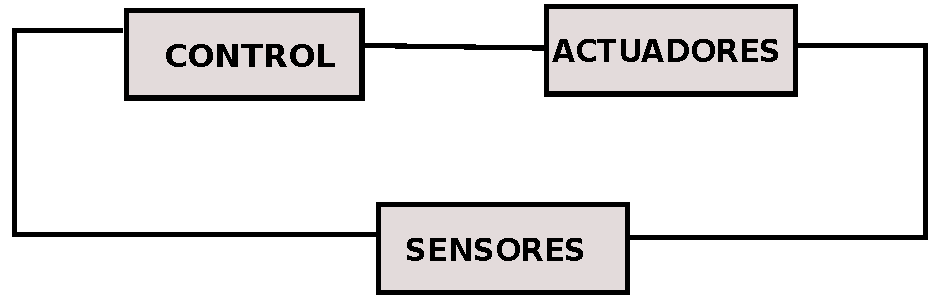
\includegraphics[width=3.0in]{imagen3.pdf}

%\caption{Marcas en cada robot}
\label{fig_mar}
\end{figure}

%%%%%%%%%%%%%%% ACA PUEDE IR ESA TABLA DEL LIBRO
 \subsection{Redes Neuronales}
 Las redes neuronales artificiales son estructuras paralelas las cuales se acercan al comportamiento de las redes neuronales humanas. Estan compuestas por neuronas  interconectadas mediantes axones donde varias neuronas pueden formar una capa (si se tratara de una red neuronal multicapa), y varias capas formar una neurona.\\
 Podemos explicar una red neuronal con salida binaria con el siguiente grafico:\\
 \begin{figure}
\centering
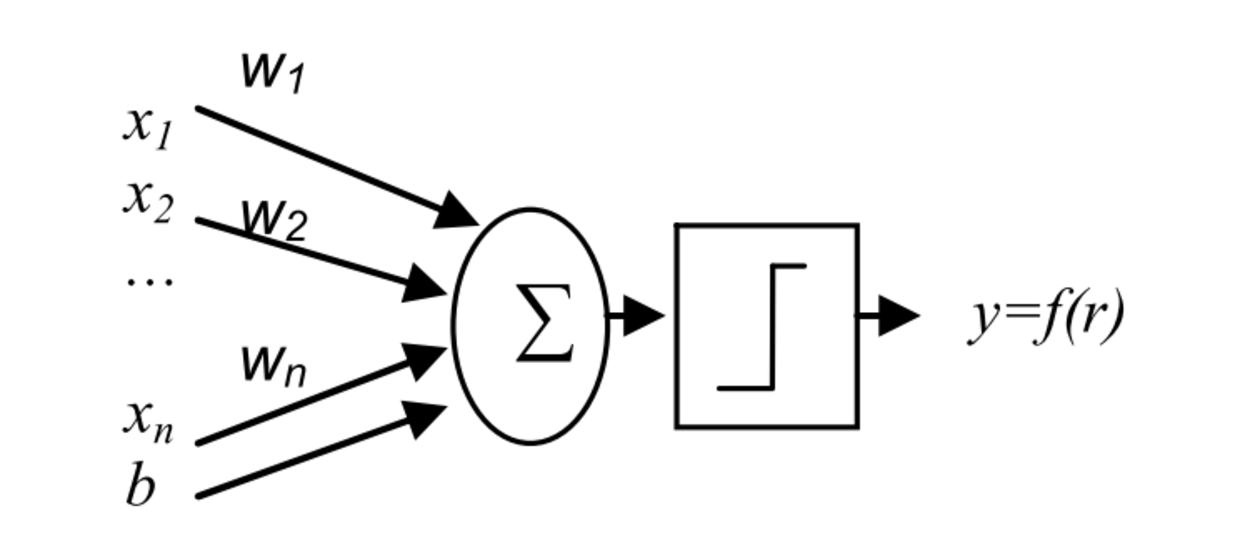
\includegraphics[width=3.0in]{imagen4.pdf}

%\caption{Marcas en cada robot}
\label{fig_mar}
\end{figure}
Donde $x_1,x_2,x_3,...,x_n$ son las entradas para la red neuronal,$w_1,w_2,w_3,...,w_n$  son los pesos sinapticos, y $b$ es un factor de polarizaci\'on. El resultado final de la funci\'on se calcular asi: 
\begin{equation}
r= \sum_{i=1}^{n}x_iw_i+b
\end{equation}
El resultado de esta ecuaci\'on  nos dar\'a 1 o 0 y si se tratara de una red multicapa este seria la entrada para otra red neuronal.\cite{art_red1}

 \subsection{Procesamiento de Imagenes}
El procesamiento de imagenes es utilizado para mejorar las imagenes,prepararlas correctamente para un analisis por parte de m\'aquinas. Consta de 4 procesos basicamente.\cite{art_red1}
\begin{enumerate}
\item Preprocesamiento: Son operaciones para adaptar la informaci\'on de una imagen y tenerla lista para el siguiente paso. Por ejemplo cambiar el brillo, reducir ruido.
\item Segmentacion: Separar la imagen en partes de las cuales se pueda hacer un analisis independiente.
\item Deteccion de objetos y clasificacion: Determinar cual objetos es cual.
\item Analisis de Imagen Obtener Informacion de alto nivel acerca de la imagen.
\end{enumerate}
 \begin{figure}
	\centering
	
\includegraphics[width=3.0in]{imagen5.pdf}
	
	%%\label{fig_mar}
\end{figure}
% \subsection{Vision Artificial}
 %\subsection{Seguimiento de Objetos}
\section{PROPUESTA}
Se propone un abordaje basado en la t\'ecnicas de procesamiento de imagenes que servir\'an para implementar el sistema de visi\'on global, el cual tendr\'a como salida la posici\'on y orientaci\'on actual en cada frame del robot. Luego de este proceso se utilizar\'a una red neuronal  que aprender\'a de los estados y las posiciones y predecir\'a los siguientes estados para hacerle el seguimiento. El esquema se presenta en la figura 4.1: \\
	\begin{figure}
	\centering
	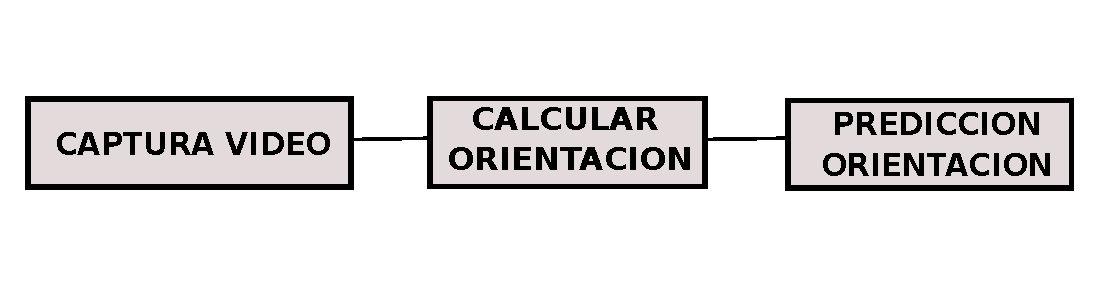
\includegraphics[width=2.5in]{esquema.pdf}
	
	\caption{Esquema del Sistema}
	\label{fig_mar}
\end{figure}
\subsection{Sistema de Visi\'on}
Para esto utilizamos marcas encima de los robots, las cuales nos dan mas facilidades para realizar la identificaci\'on de cada robot como se muestra en la Figura 4.2.
	\begin{figure}
	\centering
	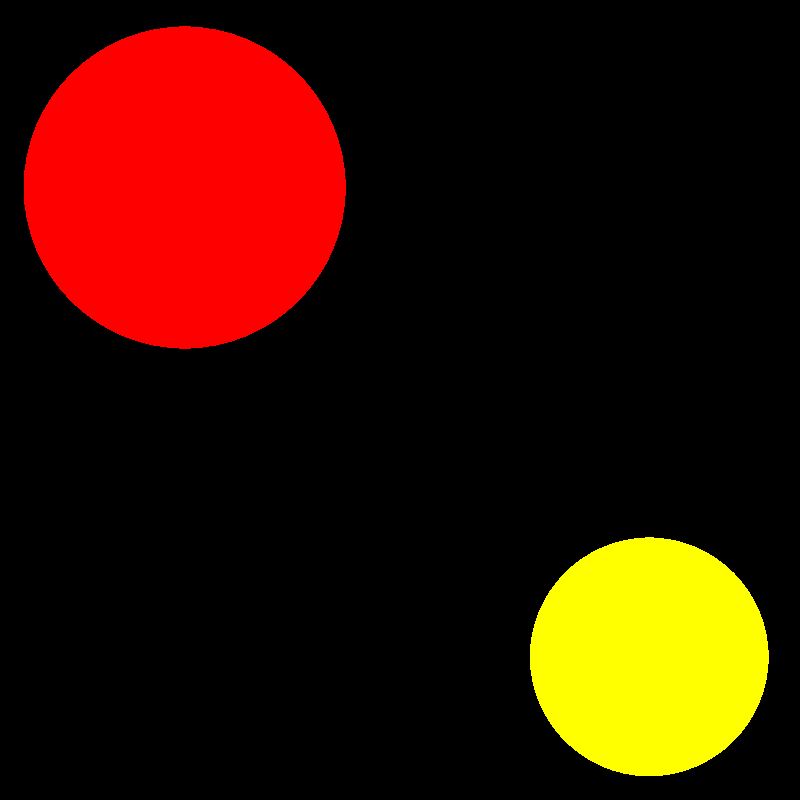
\includegraphics[width=2.5in]{imagen1.pdf}
	
	\caption{Marcas en cada robot}
	\label{fig_mar}
\end{figure}
En el sistema de vision proponemos utilizar los m\'etodos de el filtro de Gauss y la transformada de Hough. Para realizar esto utilizamos la libreria de OpenCv, la cual nos da soporte para primero aplicar un filtro de gauss para eliminar el ruido en nuestra imagen, luego convertimos nuestra imagen a la escala de grises, y finalmente aplicamos la transformada de Hough para obtener los c\'irculos en la imagen, cuyos centros tambien son hallados.\\
Una vez hallados los centros y radios de cada circulo procedemos a realizar el calculo de la ubicacion de nuestro robot, el cual utilizara unos circulos marcados como se muestra en la Fig  \ref{fig_cir}. Entonces como tenemos dos circulos de ubicacion conocida procedemos a aplicar el metodo  que nos dice que la posicion basado en esos dos circulos estara en el punto medio de la recta que une los dos centros  $c_i$ y $c_j$ de los dos circulos \cite{kelson_glo}. Entonces aplicamos punto medio entre los dos centros de los circulos:
\begin{equation}
x=\frac{x_1+y_2}{2} \qquad; y=\frac{y_1+y_2}{{2}}
\end{equation}

Una vez hallada la posicion actual del robot procedemos a hallar la orientacion con respecto al eje inicial del la imagen, de la misma forma utilizamos un metodo ya utilizado anterioremente,  el cual consiste en comparar los puntos centrales y con su tangente hallar la orientacion (angulo)\cite{kelson_glo}. El angulo $\theta$ de orientacion seria dado por:
\begin{equation}
\theta=arctan(\frac{y_1-y_2}{x_1-x_2} )
\end{equation}

\begin{figure}
\centering
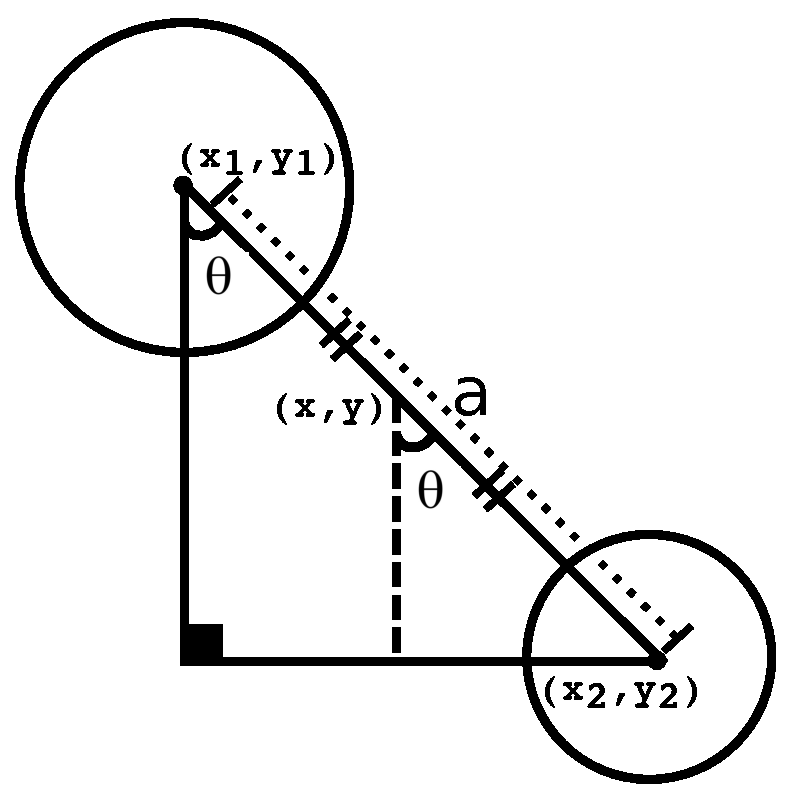
\includegraphics[width=2.5in]{imagen2.pdf}
\caption{C\'alculo de la posici\'on}
\label{fig_cir}
\end{figure}
Asi ya tenemos la posici\'on actual en cada frame y la orientaci\'on que sigue cada robot, y estamos preparados para darle estos par\'ametros a la red neuronal  y se pueda predecir su siguiente posici\'on.


\subsection{Seguimiento del Objeto}
Para realizar el seguimiento utilizaremos una Red Neuronal de Base Radial, la cual consiste en una red con una  capa de unidades ocultas, conectadas a las entradas y una neurona de salida, con transmicion directa (feedforward), donde las funciones de transferencia entre nodos (o neurones) son funciones simetricas radialmente. La estructura de la Red RBF es similar a la de la figura 4.4.
\begin{figure}
\centering
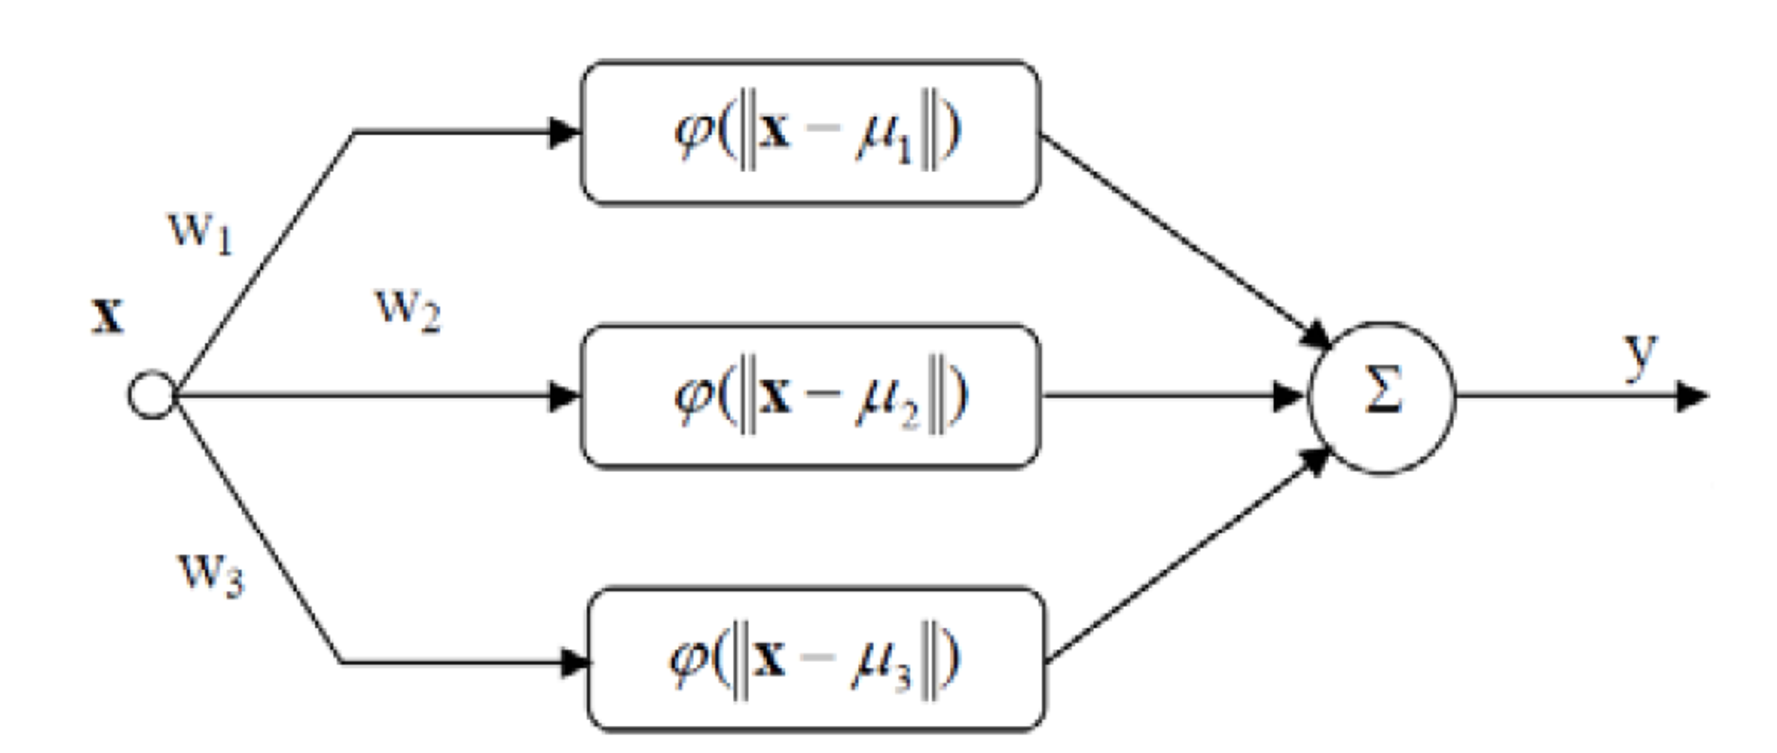
\includegraphics[width=2.5in]{RBF.pdf}
\caption{Red Neuronal de Base Radial }
\label{fig_cir}
\end{figure}

La salida para una red RBF, viene dada por: 
\[
\sum_{i=1}^{M}W_{i}\varphi(||x-\mu_i||)
\]

Donde $\varphi$ representa la funcion simetrica radialmente.
El aprendizaje en una red RBF debe ser basado en el minimizar el error, bajo la siguiente ecuacion.
\[
\sum_{p=1}^{P}(z_p-y_p)
\]
Donde $z_p$ es el valor conocido como salida, en nuestro caso la orientacion en el tiempo $t+1$, y $y_p$ es el valor de la salida de la red.\\
A esta igualdad le aplicamos el metodo de gradiente y la funcion Gaussiana,  luego de realizar los reemplazos correspondientes, nos queda que la variacion  del peso $w_i$ es como en la figura 4.5:\\
\begin{figure}
\centering
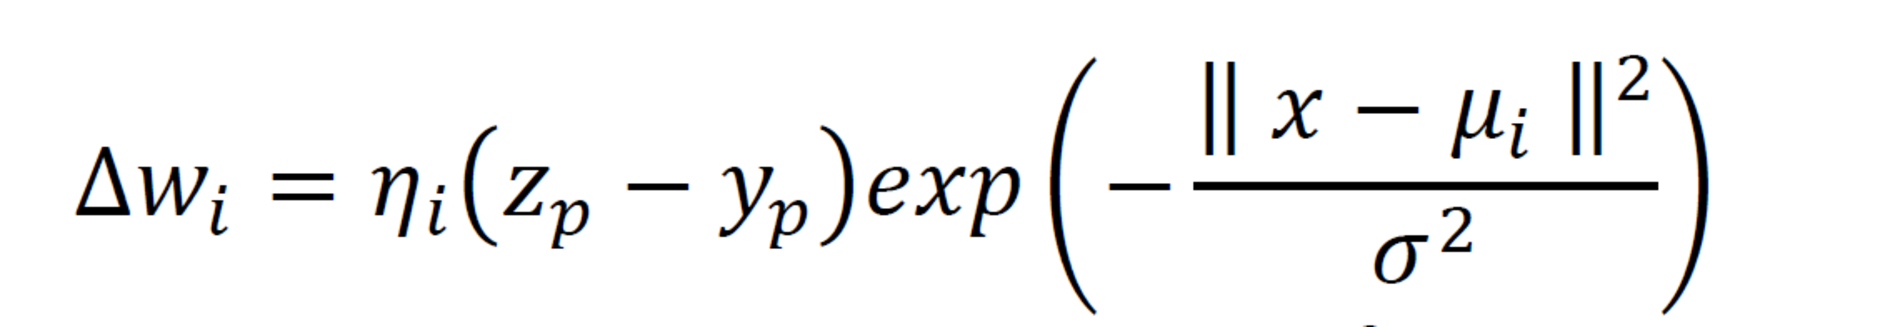
\includegraphics[width=2.5in]{eq1.pdf}
\caption{Variacion de los pesos $w_i$ }
\label{fig_cir}
\end{figure}
y para los centros quedaria como en la figura 4.6:\\
\begin{figure}
\centering
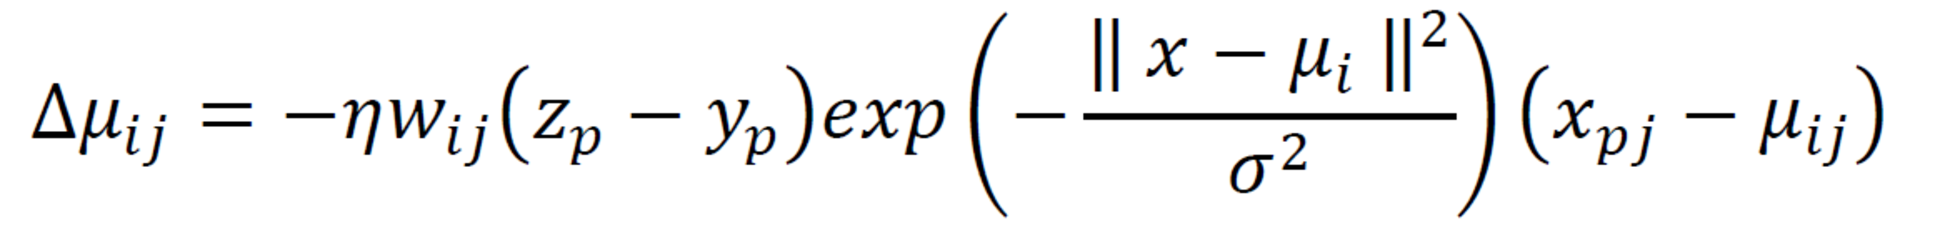
\includegraphics[width=2.5in]{eq2.pdf}
\caption{Variacion de los pesos $w_i$ }
\label{fig_cir}
\end{figure}

\section{Evaluaci\'on}
\subsection{Sistema de Visi\'on}
Utilizamos un robot del kit de robotica \textit{Robo Robo},  el cual fue programado para que se mueva aleatoriamente, ademas utilizamos una computadora Intel Core 2 Duo, bajo el Sistema Operativo Ubuntu 12.04. La camara que se utilizo fue una camara \textit{Logitech c210}, y se trabajo aproximadamente a 26 cuadros por segundo.\\
Se ha hecho pruebas con el sistema de visi\'on el cual encuentra los c\'irculos de las marcas sobre los robots, esto es realizado con la transformada de Hough utilizada del \textit{Opencv 2.4.6}, ademas se puede apreciar que al momento de capturar la imagen se muestra tambien la posicion actual del robot y la orientacion.\\
 Esto se hace para generar un archivo \textit{.dat} el cual servira como datos de entradas para nuestra red neuronal.
\begin{figure}
	\centering
	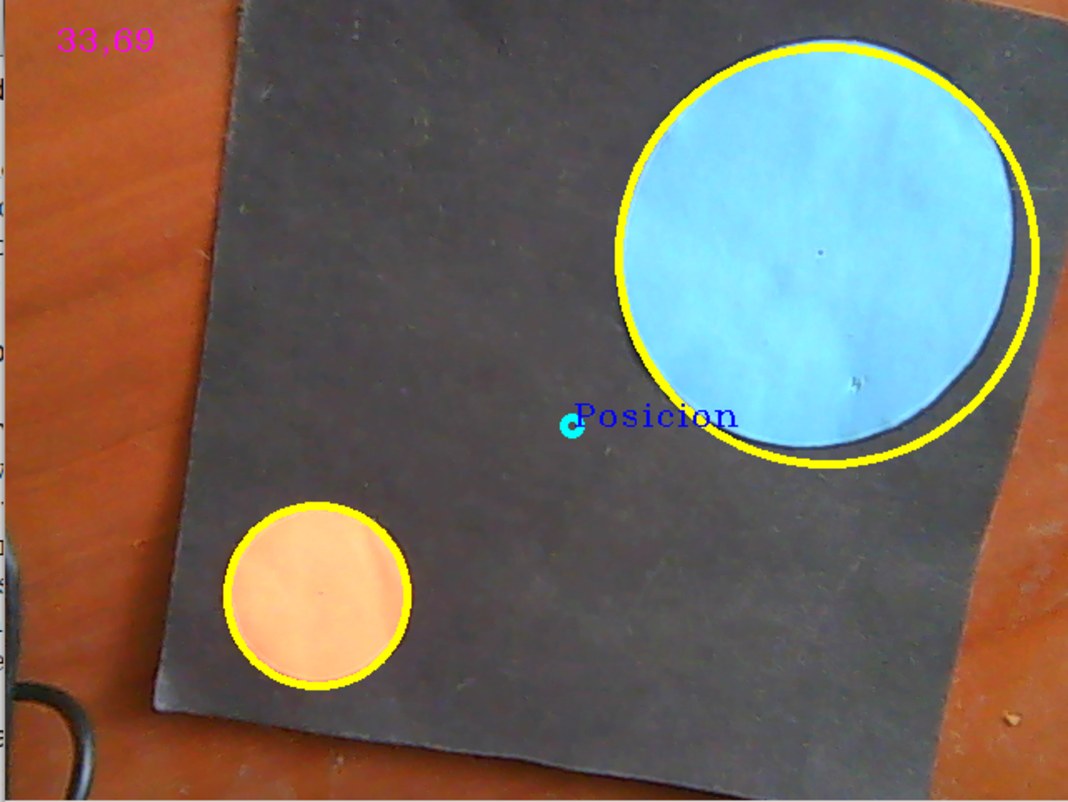
\includegraphics[width=2.5in]{visi.pdf}
	
	\caption{Ubicacion de los circulos}
	\label{fig_mar}
\end{figure}
\subsection{Seguimiento del Objeto}
Como  ya se menciono anteriormente utilizamos los archivos generados por el sistema de vision para nuestro algoritmo de seguimiento, al realizar las comparaciones sobre las salidas generadas por la red y las salidas entregadas por nosotros obtuvimos la la figura 5.2 :
\begin{figure}
	\centering
	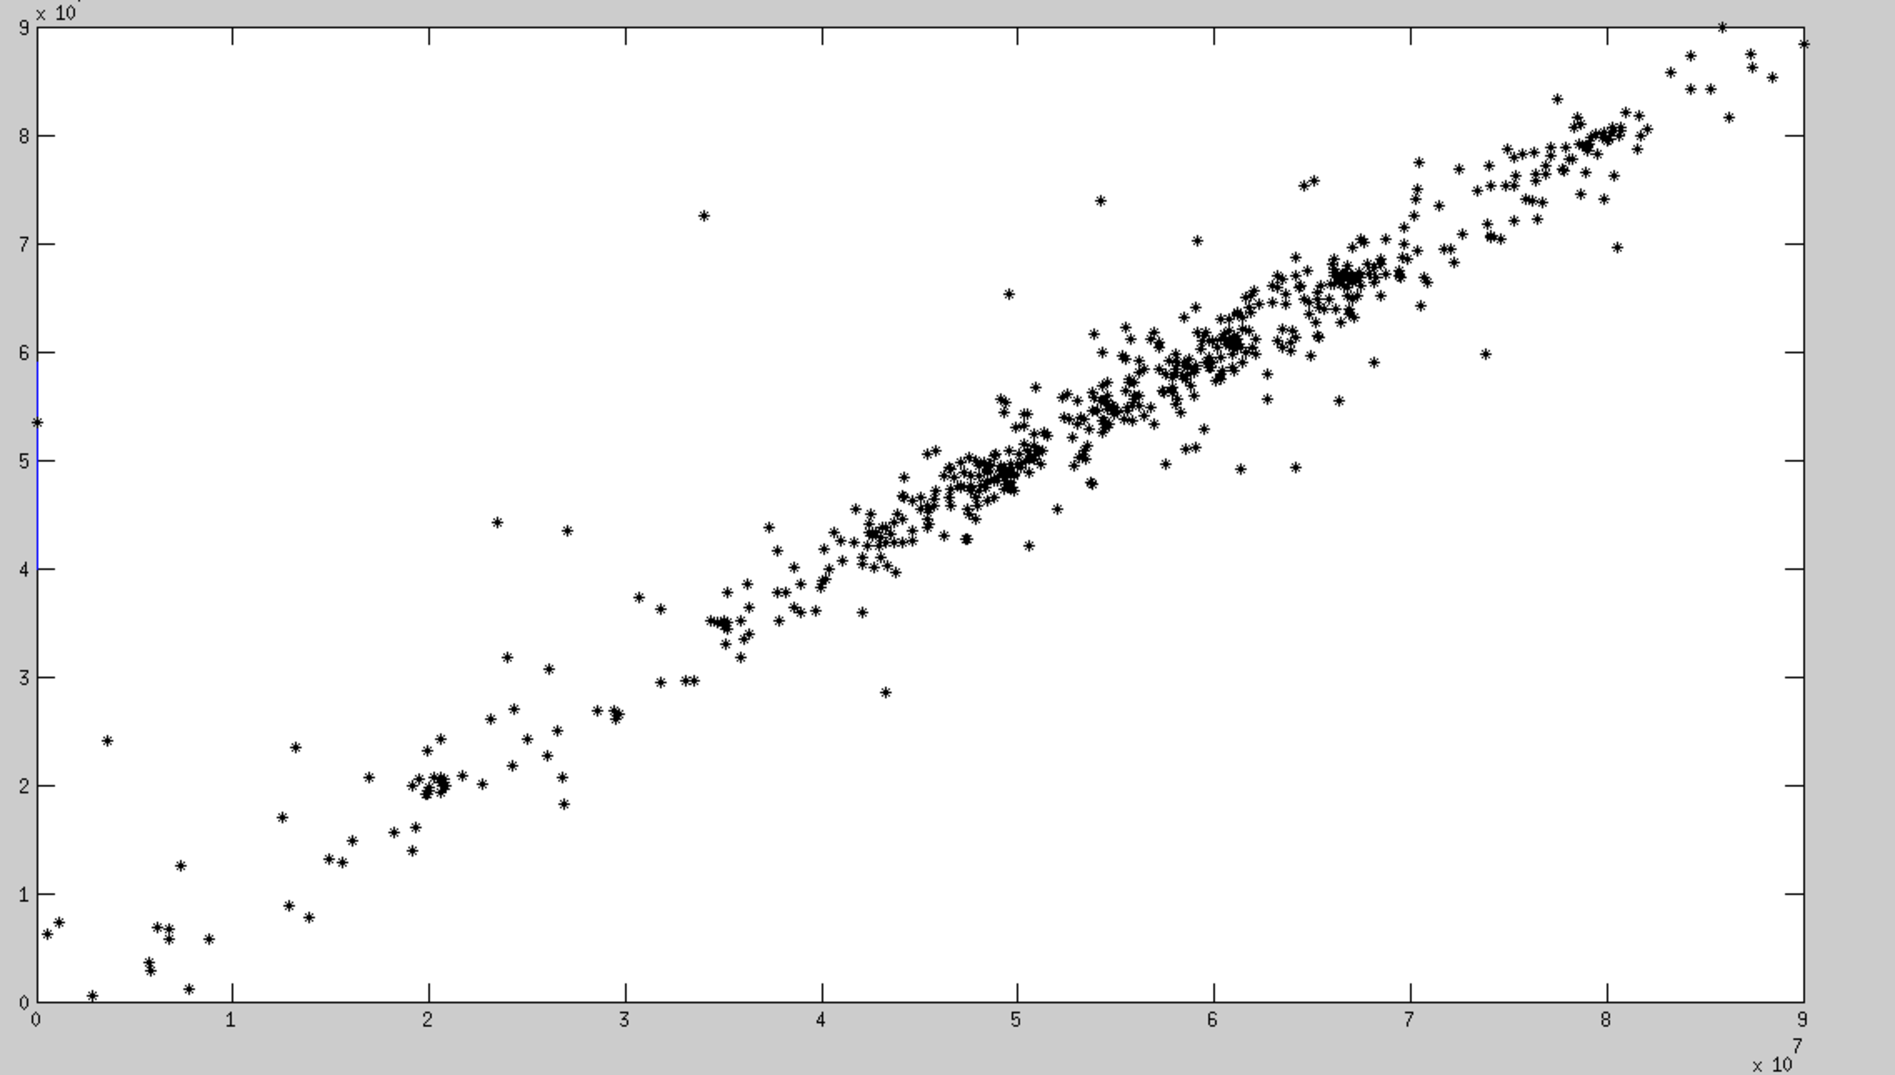
\includegraphics[width=2.5in]{salidaRBF.pdf}
	\caption{Salidas de la red RBF}
	\label{fig_mar}
\end{figure}
En el eje $x$ se pusieron las orientaciones otorgadas por el sistema de vision, y en el eje y se puso las salidas que nos da nuestro sistema de prediccion, por el grafico nos dijamos que las predicciones estan muy cercanas a los valores originales.
Para comparar nuestros resultados utilizamos una red Neuronal del tipo Focused Time Delay, esta tipo de red neuronal dinamica tiene la propiedad de volver a valores anteriores (\textit{delay}) para alimentar a las nuevas salidas, en este caso se dividio toda las muestras en partes para el entrenamiento, para la validacion y para las pruebas, a continuacion mostramos el la misma grafica(figura 5.3). En este caso el algoritmo fue implementado utilizando el  \textit{Neural Network Toolbox} del MatLab, el cual nos dio este resultado mostrado en la figura 5.3 :
\begin{figure}
	\centering
	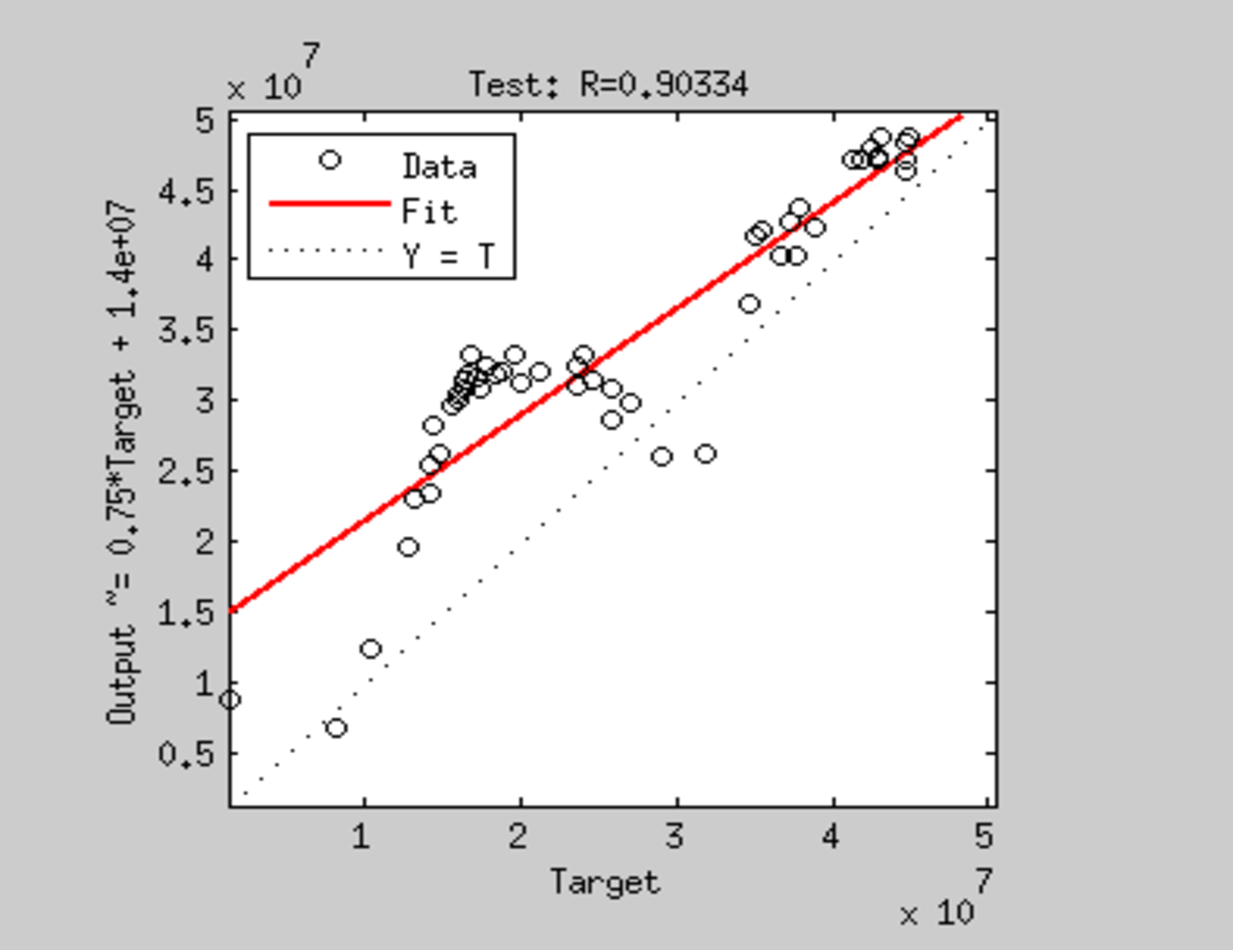
\includegraphics[width=2.5in]{salidaNAR.pdf}
	\caption{Salida de la Red Focused Time Delay}
	\label{fig_mar}
\end{figure}

%\section{IMPLEMENTACION}
%
\section{Conclusiones y Recomendaciones}
\begin{itemize}
\item El Sistema de Vision fue implementado utilizando la biblioteca OpenCV y se uso la IDE de programacion  QT Creator.
\item Se utilizo el \textit{Neural Network Toobox} para realizar la comparacion de nuestro algoritmo de seguimiento.
\item Para comparar se utilizo red Neuronal Dinamica la cual nos permitia utilizar valores anteriores a nuestro actual valor de entrada para tener una mejor salida, sin embargo de acuerdo a las graficas obtenidas hay mejor precision con el modelo de red RBF..
\item Las graficas obtenidas por el Matlab nos indican que nuestra red tiene un buen desempeño, ya que los datos comparados no estan muy separados entre si.
\end{itemize}
%\subsection{Aportaciones}
%\subsection{Limitaciones}
%\subsection{Conclusiones}
%\subsection{Recomendaciones}
%\subsection{Trabajos Futuros}

% conference papers do not normally have an appendix
% use section* for acknowledgement
%\section*{Agradecimientos}
%The authors would like to thank...

% trigger a \newpage just before the given reference
% number - used to balance the columns on the last page
% adjust value as needed - may need to be readjusted if
% the document is modified later
%\IEEEtriggeratref{8}
% The "triggered" command can be changed if desired:
%\IEEEtriggercmd{\enlargethispage{-5in}}

% references section

% can use a bibliography generated by BibTeX as a .bbl file
% BibTeX documentation can be easily obtained at:
% http://www.ctan.org/tex-archive/biblio/bibtex/contrib/doc/
% The IEEEtran BibTeX style support page is at:
% http://www.michaelshell.org/tex/ieeetran/bibtex/
%\bibliographystyle{IEEEtran}
% argument is your BibTeX string definitions and bibliography database(s)
%\bibliography{IEEEabrv,../bib/paper}
%
% <OR> manually copy in the resultant .bbl file
% set second argument of \begin to the number of references
% (used to reserve space for the reference number labels box)
%\bibliography{biblio.bib}

\begin{thebibliography}{1}
\bibitem{Morales_g}
E.F.Morales and L.E. Sucar, \emph{Robots y su importancia para M\'exico}, 1st~ed.\hskip 1em plus
  0.5em minus 0.4em\relax Mexico, Instituto Nacional de Astrofisica, Optica y Electronica, Komputer Sapiens 2009 
  
\bibitem{Garcia_g}
Pablo Garcia-Robledo and Jesus Torrijos \emph{Robots de Seguridad y Defensa}\hskip 1em plus
  0.5em minus 0.4em\relax  Espa\~na, Universidad Politecnica de Madrid, 2010

\bibitem{Vasquez_g}
J.A. Garcia and L.A. Vasquez  \emph{Los Robots en el Sector Agr\'icola}\hskip 1em plus
  0.5em minus 0.4em\relax  España, Departamento  De automatica, Ingenieria Electronica e Informatica Industrial, Universidad Politecnica de Madrid,2010

\bibitem{Baltes_g}
Jacky Baltes and John Anderson \emph{Intelligent Global Vision for Teams of Mobile Robots, Mobile Robots:Perception \& Navigation, Sascha Kolski (Ed.), ISBN: 3-86611-283-1, InTech,Available from: http://www.intechopen.com/books/mobile-robots-perception-navigation/intelligent-global-vision-for-teams-of-mobile-robots}, 1st ed.\hskip 1em plus
  0.5em minus 0.4em\relax Pro Literatur Verlag, Germany/ARS Austria 2007.

\bibitem{Brezac_g}
Misel Brezac, Ivan Petrovic and Edouard Ivanjko, \emph{Robust and accurate global vision system for real time tracking of multiple mobile robots,Robotics and Autonomous Systems 56 (2008) 213-230.}\hskip 1em plus
  0.5em minus 0.4em\relax Elsiever, 2008

\bibitem{acharya_g}
Tinku Acharya and Ajoy K. Ray, \emph{Image Processing Principles and Applications, pag. 6}, 1st ed.\hskip 1em plus
  0.5em minus 0.4em\relax  B. Michaelis and G. Krell (Eds.): DAGM 2003, LNCS 2781, pp. 591–599, Springer-Verlag Berlin Heidelberg 2003.

\bibitem{kelson_glo}
Kelson Romulo Teixeira Aires, Pablo Javier Alsina, Adelardo Adelino Dantas de Medeiros , \emph{A GLOBAL VISION SYSTEM FOR MOBILE MINI-ROBOTS} ed.\hskip 1em plus 0.5em minus 0.4em\relax SIMPÓSIO BRASILEIRO DE AUTOMAÇÃO INTELIGENTE, 5, Canela, 2001

\bibitem{chabra_glo}
Manu Chhabra, Anusheel Nahar, Nishant Agrawal, Tamhant Jain,Amitabha Mukerjee, Apurva Mathad and Siddhartha Chaudhuri, \emph{Novel Approaches to Vision and Motion Control for Robot Soccer} ed.\hskip 1em plus 0.5em minus 0.4em\relax Proceedings  of the National Conference on Advance Manufacturing and Robotics, India 2004 


\bibitem{ball_glo}

Ball, David and Wyeth, Gordon and Nuske, Stephen, \emph{A global vision 
system for a robot soccer team} ed.\hskip 1em plus 0.5em minus 0.4em\relax SAustralasian Conference on Robotics and Automation, 6-8 December 2004, Canberra

\bibitem{clau_glo}
Gönner, Claudia and Rous, Martin and Kraiss, Karl-Friedrich, \emph{Real-Time Adaptive Colour Segmentation for the RoboCup Middle Size League} ed.\hskip 1em plus 0.5em minus 0.4em\relax RoboCup 2004: Robot Soccer World Cup VIII, Springer Berlin Heidelberg

 \bibitem{nummiaro_mot}
Kajta Nummiaro, Esther Koller-Meier, Tomas Svoboda, Daniel Roth, and Lucas Van Gool and Ajoy K. Ray, \emph{Color-Based Object Tracking in Multi-camera Environments}, 1st ed.\hskip 1em plus
  0.5em minus 0.4em\relax  B. Michaelis and G. Krell (Eds.): DAGM 2003, LNCS 2781, pp. 591–599, Springer-Verlag Berlin Heidelberg 2003 
  
 \bibitem{morioka_mul}
Kazuki Morioka, Silvester Kovacs, Peter Korondp, Joo-Hoo Lee and Hideki Hashimoto, \emph{Adaptative camera selection based on fuzzy automaton for object tracking in a Muticamera System} ed.\hskip 1em plus
  0.5em minus 0.4em\relax Journal of Engineering Annals of Faculty of Engineering Hunedoara, 2008 
  
 \bibitem{Dick_mot}
Anthony R. Dick and Michael J. Brooks, \emph{A Stochastic Approach to Tracking Objetcs Across Multiple  Cameras} ed.\hskip 1em plus 0.5em minus 0.4em\relax Springer -Verlag Berlin Heidelberg, 2004
 
\bibitem{garcia_mot}
Renato F. Garcia, Pedro M. Shiroma, Luiz Chaimowicz, Mario F.M. Campos, \emph{Um Arcabouco para Localizacao de Enxames de Robos} ed.\hskip 1em plus 0.5em minus 0.4em\relax Universidade Federal de Minas Gerais, Belo Horizonte,VIII Simposio Brasileiro de Automacao Inteligente, Brazil 2007

\bibitem{kumar_mot}
Piyush Kumar Rai, Kamal Tiwari, Prithwijit Guha and Amitabha Mukerjee , \emph{A cost-Effective Multiple Camera Vision System using Firewire Cameras and Software Synchronization} ed.\hskip 1em plus 0.5em minus 0.4em\relax IIT Kanpur, UP, India 2003. 

%\bibitem{karabiber_mot}
%Fethullah Karabiber,  Paolo Arena, Luigi Fortuna,  Sabestiano De Fiore,  Guido Vagliasindi and Sabri Arik , \emph{Implementation of a Moving Target Tracking Algorithm Using Eye-RIS Vision System on a Mobile Robot} ed.\hskip 1em plus 0.5em minus 0.4em\relax Springer Science+Business Media, LLC 2010 

\bibitem{hossiein_mul}
Amir Hossein Khalili and Shohreh Kasaei , \emph{Object Modeling for Multicamera Correspondence Using Fuzzy Region Color Adjacency Graphs} ed.\hskip 1em plus 0.5em minus 0.4em\relax Springer Berlin Heidelberg, Advances in Computer Science and Engineering 2009 


\bibitem{oto_mul}
Emre Oto, Frances Lau, and Hamid Aghajan , \emph{Color-Based Multiple Agent Tracking for
Wireless Image Sensor Networks} ed.\hskip 1em plus 0.5em minus 0.4em\relax Proceedings of the 8th international conference on Advanced Concepts For Intelligent Vision Systems,Springer-Verlag,2006

%\bibitem{yaldaz_mot}
%Yildiz, Alparslan and Akgul, YusufSinan , \emph{A Fast Method for Tracking People with Multiple Cameras} ed.\hskip 1em plus 0.5em minus 0.4em\relax Trends and Topics in Computer Vision,Springer Berlin Heidelberg,2012

%\bibitem{Santos_art}
%Santos, Thiago T. and Morimoto, Carlos H. , \emph{Multiple camera people detection and tracking using support integration} ed.\hskip 1em plus 0.5em minus 0.4em\relax Journal Pattern Recognition Letters,SElsevier B.V.,2011

%\bibitem{Hofman_art}
%Hofmann, M., Wolf, D., \& Rigoll, G. (2013).  \emph{Hypergraphs for Joint Multi-view Reconstruction and Multi-object Tracking}. \hskip 1em plus 0.5em minus 0.4em\relax 2013 IEEE Conference on Computer Vision and Pattern Recognition, 3650–3657. doi:10.1109/CVPR.2013.468

%\bibitem{Leal_art}
%L. Leal-Taixe, G. Pons-Moll, and B. Rosenhahn. \emph{Branch-and-price global optimization for multi-view multi-object tracking}. \hskip 1em plus 0.5em minus 0.4em\relax In 2012 IEEE Conference on Computer Vision and Pattern Recognition, June 2012
%
%\bibitem{Bilir_art}
%Bilir, S. C., \& Yemez, Y. (2012).\emph{ Non-rigid 3D shape tracking from multiview video}. \hskip 1em plus 0.5em minus 0.4em\relax  Computer Vision and Image Understanding, 116(11), 1121–1134. doi:10.1016/j.cviu.2012.07.001

%\bibitem{Greek_art}
%Tzevanidis, K., \& Argyros, A. (2011).  \emph{Unsupervised learning of background modeling parameters in multicamera systems}.  \hskip 1em plus 0.5em minus 0.4em\relax Computer Vision and Image Understanding, 115(1), 105–116. doi:10.1016/j.cviu.2010.09.003
\bibitem{lib_rob1}
Antonio Barrientos, Luis Felipe Pe\~nin, Carlos Balaguer \& Rafael Aracil (1997). \emph{Fundamentos de Rob\'otica }.  \hskip 1em plus 0.5em minus 0.4em\relax McGraw-Hill/ Interamericana Espa\~na. ISBN 84-481-0815-9

\bibitem{lib_rob2}

Bruno Siciliano, Lorenzo Sciavicco, Luigi Villani \& Giuseppe Oriolo (2009). \emph{Robotics Modelling, Plannig and Control }.  \hskip 1em plus 0.5em minus 0.4em\relax Springer-Verlag London Limited. ISBN 978-1-84628-641-4

\bibitem{art_red1}

Juan, R. Q., \& Chacón, A. (2011). \emph{Redes neuronales artificiales para el procesamiento de imágenes , una revisión de la última década}.  \hskip 1em plus 0.5em minus 0.4em\relax Revista de Infenieria Electrica, Electronica y Computacion ISSN 1870-9532
\end{thebibliography}




% that's all folks
\end{document}


